\def\documentauthor{Carlos Salinas}
\def\hwnum{1-10}
\def\documenttitle{MA166: Solutions to Homework {\hwnum}}
\def\shorttitle{MA166-HW-\hwnum-Sols}
\def\coursename{MA166}
\def\documentsubject{calculus ii}
\def\authoremail{salinac@purdue.edu}

\documentclass[article,oneside,10pt]{memoir}
\usepackage{geometry}
\usepackage[dvipsnames]{xcolor}
\usepackage[
    breaklinks,
    bookmarks=true,
    % colorlinks=true,
    pageanchor=false,
    linkcolor=black,
    anchorcolor=black,
    citecolor=black,
    filecolor=black,
    menucolor=black,
    runcolor=black,
    urlcolor=black,
    hyperindex=false,
    hyperfootnotes=true,
    pdftitle={\shorttitle},
    pdfauthor={\documentauthor},
    pdfkeywords={\documentsubject},
    pdfsubject={\coursename}
    ]{hyperref}

% Use symbols instead of numbers
\renewcommand*{\thefootnote}{\fnsymbol{footnote}}

%% Math
\usepackage{bm}
\usepackage{soul}
\usepackage{amsmath}
\usepackage{amssymb}
\usepackage{amsthm}
\usepackage{mathtools}
\usepackage{siunitx}

%% PDFTeX specific
\usepackage[mathcal]{euscript}
\usepackage{mathrsfs}

\usepackage[LAE,LFE,T2A,T1]{fontenc}
\usepackage[utf8]{inputenc}
\usepackage[farsi,french,german,spanish,russian,english]{babel}
\babeltags{fr=french,
           de=german,
           en=english,
           es=spanish,
           pa=farsi,
           ru=russian
           }
\def\spanishoptions{mexico}

\selectlanguage{english}

\newcommand{\textfa}[1]{\beginR\textpa{#1}\endR}

\usepackage{cmap}
\usepackage{CJKutf8}
\newcommand{\textkr}[1]{\begin{CJK}{UTF8}{mj}#1\end{CJK}}
\newcommand{\textjp}[1]{\begin{CJK}{UTF8}{min}#1\end{CJK}}
\newcommand{\textzh}[1]{\begin{CJK}{UTF8}{bsmi}#1\end{CJK}}

\usepackage{graphicx}
\graphicspath{{figures/}}

% Misc
\usepackage{microtype}
\usepackage{multicol}
\usepackage[inline]{enumitem}
\usepackage{listings}
\usepackage{mleftright}
\mleftright

%% Theorems and definitions
%% remove parentheses
% \makeatletter
% \def\thmhead@plain#1#2#3{%
%   \thmname{#1}\thmnumber{\@ifnotempty{#1}{ }\@upn{#2}}%
%   \thmnote{ {\the\thm@notefont#3}}}
% \let\thmhead\thmhead@plain
% \makeatother

\theoremstyle{plain}
\newtheorem{theorem}{Theorem}
\newtheorem{proposition}[theorem]{Proposition}
\newtheorem{corollary}[theorem]{Corollary}
\newtheorem{claim}[theorem]{Claim}
\newtheorem{lemma}[theorem]{Lemma}
\newtheorem{axiom}[theorem]{Axiom}

\newtheorem*{corollary*}{Corollary}
\newtheorem*{claim*}{Claim}
\newtheorem*{lemma*}{Lemma}
\newtheorem*{proposition*}{Proposition}
\newtheorem*{theorem*}{Theorem}

\theoremstyle{definition}
\newtheorem{definition}{Definition}
\newtheorem{example}{Examples}
\newtheorem{examples}[example]{Examples}
\newtheorem{exercise}{Exercise}[chapter]
\newtheorem{problem}[exercise]{Problem}

\newtheorem*{example*}{Example}
\newtheorem*{exercise*}{Exercise}
\newtheorem*{problem*}{Problem}

\theoremstyle{remark}
\newtheorem{remark}{remark}
\newtheorem{remarks}{Remarks}

\newtheorem*{remark*}{remark}
\newtheorem*{remarks*}{Remarks}


%% Redefinitions & commands
\newcommand{\nle}{\ensuremath{\not<}}
\newcommand{\nge}{\ensuremath{\not>}}
\newcommand{\nsubset}{\ensuremath{\not\subset}}
\newcommand{\nsupset}{\ensuremath{\not\supset}}
\newcommand\minus{\ensuremath{\null\smallsetminus}}
\renewcommand\qedsymbol{\ensuremath{\null\hfill\blacksquare}}

%% Commands and operators
\DeclareMathOperator{\comp}{comp}
\DeclareMathOperator{\proj}{proj}

\newcommand{\diff}{\,\mathrm{d}}

\newcommand{\bbC}{\mathbb{C}}
\newcommand{\bbN}{\mathbb{N}}
\newcommand{\bbQ}{\mathbb{Q}}
\newcommand{\bbR}{\mathbb{R}}
\newcommand{\bbZ}{\mathbb{Z}}

\newcommand{\bfu}{\mathbf{u}}
\newcommand{\bfv}{\mathbf{v}}
\newcommand{\bfw}{\mathbf{w}}

\begin{document}
\author{\href{mailto:\authoremail}{\documentauthor}}
\title{\documenttitle}
\date{\today}
\maketitle
% \chapter{Solutions to Homework}
These are solutions the assigned problems from Stewart's \emph{Calculus,
  Early Transcendentals, 7th ed.}\,from the
\href{https://www.math.purdue.edu/academic/files/courses/2016spring/MA16600/166assignr1.pdf}{assignment
  sheet}. I plan to keep updating the solutions sheet as the semester goes
on.
\begin{problem}[Stewart \S{12.1}, Exercise 6]
\begin{enumerate}[label=(\alph*)]
\item What does the equation $x=4$ represent in $\bbR^2$? What does it
  represent in $\bbR^3$? Illustrate with a sketches.
\item What does the equation $y=3$ represent in $\bbR^3$? What does $z=5$
  represent? What does the pair of equations $y=3$, $z=5$ represent? In
  other words, describe the set of points $(x,y,z)$ such that $y=3$ and
  $z=5$. Illustrate with a sketch.
\end{enumerate}
\end{problem}
\begin{proof}[Solution]
In such problems, your first instinct should be to ask yourself ``What is a
point on the equation I am given?.''

(a) Let us begin by making a table of values of $x=4$ in $\bbR^2$:
\begin{center}
\begin{tabular}{|c|c|}
\hline
$x$&$y$\\
\hline
4&0\\
4&1\\
4&-1\\
4&1000\\
\hline
\end{tabular}.
\end{center}
Recognize the pattern? In fact, for any value of $y$ that we choose, $x$
will always be $4$ so the equation represents a \ul{vertical line which
  perpendicular to the $x$-axis, and touching the $x$-axis at the point
  $(0,4)$.}

We can use the same method to figure out what this equation, $x=4$,
represents in $\bbR^3$:
\begin{center}
\begin{tabular}{|c|c|c|}
\hline
$x$&$y$&$z$\\
\hline
4&0&0\\
4&1&0\\
4&0&1\\
4&1&1\\
\hline
\end{tabular}.
\end{center}
If you know some linear algebra, we have enough
\href{https://en.wikipedia.org/wiki/Linear_independence}{linearly
  independent} vectors to span a \ul{plane}. If you don't know any
linear algebra, just note that if we choose any values for $y$ and $z$ the
point $(4,y,z)$ will still be on the equation $x=4$. Hence, the equation
$x=4$ represents a plane \ul{perpendicular to $x$-axis at the
  point $(4,0,0)$.}
\\\\
(b) Again, we may repeat the previous strategy to solve this problem
$y=3$,i.e., we make a table with points in the equation $y=3$
\begin{center}
\begin{tabular}{|c|c|c|}
\hline
$x$&$y$&$z$\\
\hline
$0$&$3$&$0$\\
$1$&$3$&$0$\\
$1$&$3$&$-1$\\
\hline
\end{tabular}.
\end{center}
Again, we see that no matter what value of $x$ and $z$ we pick, the point
$(x,3,z)$ will always be in the equation $y=3$. Hopefully, you can see why
this equation represents a \ul{plane perpendicular to the $y$-axis at the
  point $(0,3,0)$}.

Hopefully you are able to see the pattern now and can tell me all on your
own what the equation $z=5$ represents in $\bbR^3$. Right! It will be a
\ul{plane perpendicular to the $z$-axis and touching the $z$-axis at the
  point $(0,0,5)$.} In fact, we can make a categorical statement about what
$x=a$ and $y=b$ or $z=c$ represent in $\bbR^3$:
\begin{definition}
Let $a$ stand-in for one of the $x$, $y$, or $z$ variables and let $b$ be
any real number. Then the equation
\begin{equation}
  \label{eq:plane}
  a=b
\end{equation}
represents a plane perpendicular to the $a$-axis and touching the $a$-axis
at the point $(b,0,0)$ (or $(0,b,0)$, or $(0,0,b)$ as it may be).
\end{definition}

Now, it is not so clear what the pair of equations $y=3$ and $z=5$, but we
can make a table and take a look at some of the values these equations take
on
\begin{center}
\begin{tabular}{|c|c|c|}
\hline
$x$&$y$&$z$\\
\hline
$-1$&$3$&$5$\\
$0$&$3$&$5$\\
$-1$&$3$&$5$\\
$1000$&$3$&$5$\\
\hline
\end{tabular}.
\end{center}
So no matter what value of $x$ we pick, the point $(x,3,5)$ will be in the
pair of equations $y=3$ and $z=5$. Hence, we can see that this pair of
equations represents a \ul{line extending in the same direction $x$-axis
  which touches the point $(0,3,5)$.} That last bit is a bit arbitrary, we
can say it touches the point $(1,3,5)$ or even $(10000,3,5)$, there is not
much else we can say since the line never touches the any of the axes, but
it does cross the $yz$-plane at the point $(0,3,5)$, which is questionably
useful.

In fact, an easier way to say this is that the pair of equations $y=3$ and
$z=5$ represents the intersection of the planes $y=3$ and $z=5$. Finding
the line where these planes intersect is equivalent to finding the points
that the pair of equations satisfy.
\end{proof}
\begin{remarks*}
In all this discussion, I failed to address one thing and that is, for
example, why the point $(0,-3,5)$ is not on the pair of equations $y=3$ and
$z=5$. Well, that is simply because we have a restriction on $y$ and $z$,
i.e., $y$ must be $3$ and $z$ must be $5$ or else we are looking at
something all together different.
\end{remarks*}

\begin{problem}[Stewart \S{12.1}, Exercise 16]
Show that the equation represents a sphere, and find its center and radius.
\[
x^2+y^2+z^2-2x-4y+8z=15.
\]
\end{problem}
\begin{proof}[Solution]
You have no doubt seen the \emph{standard equation} for a sphere of
radius $r$ centered at $\left(x_0,y_0,z_0\right)$; in case you missed it
here it is
\begin{equation}
\label{eq:sphere}
\left(x-x_0\right)^2+\left(y-y_0\right)^2+\left(z-z_0\right)^2=r^2.
\end{equation}
What is scary is that an equation of the form
\[
Ax^2+By^2+Cz^2+Dxy+Exz+Fyz+Gx+Hy+Iz+J=0
\]
is called a \href{https://en.wikipedia.org/wiki/Conic_section}{conic
  section} and if we are given an equation like the one above, we cannot
always factor it into something nice. Enough of that, our equation is
clearly an equation of a sphere (you can tell this because it does not
contain any mixed terms, i.e., terms of the form $xy$, $xz$, or $yz$) so we
can use the method of
\href{https://en.wikipedia.org/wiki/Completing_the_square}{completing the
  square} to express the equation in standard form:
\begin{align*}
x^2+y^2+z^2-2x-4y+8z&=15\\
\left(x^2-2x\right)+\left(y^2-4y\right)+\left(z^2+8z\right)&=15\\
\left(x^2-2x+1\right)-1+\left(y^2-4y+2\right)-2+\left(z^2+8z+16\right)-16&=15\\
\left(x^2-2x+1\right)+\left(y^2-4y+2\right)+\left(z^2+8z+16\right)&=15+1+2+16\\
\left(x-1\right)^2+\left(x-2\right)^2+\left(x+4\right)^2&=34\\
\end{align*}
Now that we've gotten the equation down the standard form of a sphere, we
can read off the necessary values: So the equation
\[
x^2+y^2+z^2-2x-4y+8z=15
\]
represents a \ul{sphere centered at $(1,2,4)$ with radius $\sqrt{34}$}.
\end{proof}

% p790:6,16,31,33,37,38
\begin{problem}[Stewart \S{12.1}, Exercise 31]
Describe in words the region of $\bbR^3$ represented by the inequality
\[
x^2+y^2+z^2\leq 3.
\]
\end{problem}
\begin{proof}[Solution]
  Remember the equation of our good old friend the
  \hyperref[eq:sphere]{sphere}? Well, it's not quite a sphere that we have
  but something like it. The equation we are given is indeed that of a
  sphere, but the radius is allowed to change from $0$ to $\sqrt{3}$ so it
  is in fact a union of spheres of every radius between $0$ and
  $\sqrt{3}$. In other words, it is the \ul{solid sphere (also called a
    ball) of radius $3$}.
\end{proof}

\begin{problem}[Stewart \S{12.1}, Exercise 33]
Describe in words the region of $\bbR^3$ represented by the inequality
\[
x^2+z^2\leq 9.
\]
\end{problem}
\begin{proof}[Solution]
  This looks something like the circle of radius $3$ in the $xz$-plane. In
  fact, we again have all of the circles of radius $0$ to $3$ in the
  $xz$-plane and this gives us a \ul{solid circle of radius (also called a
    disk) $3$}.
\end{proof}

\begin{problem}[Stewart \S{12.1}, Exercise 37]

\end{problem}
\begin{proof}[Solution]
\end{proof}

\begin{problem}[Stewart \S{12.1}, Exercise 38]

\end{problem}
\begin{proof}[Solution]
\end{proof}

% +12.2 beg.-Ex. 2
% p798:3,5
\begin{problem}[Stewart \S{12.2}, Exercise 3]

\end{problem}
\begin{proof}[Solution]
\end{proof}

\begin{problem}[Stewart \S{12.2}, Exercise 5]

\end{problem}
\begin{proof}[Solution]
\end{proof}

%%% Local Variables:
%%% mode: latex
%%% TeX-master: "../MA166-HW-Current"
%%% End:

% \chapter{Solutions to Homework 2}

\begin{problem}[Stewart \S{12.2}, Exercise 11]

\end{problem}
\begin{proof}[Solution]
\end{proof}

\begin{problem}[Stewart \S{12.2}, Exercise 13]

\end{problem}
\begin{proof}[Solution]
\end{proof}

\begin{problem}[Stewart \S{12.2}, Exercise 17]

\end{problem}
\begin{proof}[Solution]
\end{proof}

\begin{problem}[Stewart \S{12.2}, Exercise 19]

\end{problem}
\begin{proof}[Solution]
\end{proof}

\begin{problem}[Stewart \S{12.2}, Exercise 25]

\end{problem}
\begin{proof}[Solution]
\end{proof}

\begin{problem}[Stewart \S{12.2}, Exercise 26]

\end{problem}
\begin{proof}[Solution]
\end{proof}

% p798:11,13,17,19,25,26

\begin{problem}[Stewart \S{12.3}, Exercise 11]

\end{problem}
\begin{proof}[Solution]
\end{proof}

% p806:5,8,9
\begin{problem}[Stewart \S{12.3}, Exercise 5]

\end{problem}
\begin{proof}[Solution]
\end{proof}

\begin{problem}[Stewart \S{12.3}, Exercise 8]

\end{problem}
\begin{proof}[Solution]
\end{proof}

\begin{problem}[Stewart \S{12.3}, Exercise 9]

\end{problem}
\begin{proof}[Solution]
\end{proof}

%%% Local Variables:
%%% mode: latex
%%% TeX-master: "../MA166-HW-Current"
%%% End:

% \chapter{Solutions to Homework 3}
 % p806:20,23,25,31,34,41,43,52

%%% Local Variables:
%%% mode: latex
%%% TeX-master: "../MA166-HW-Current"
%%% End:

% \chapter{Solutions to Homework 4}
% p814:1,4,5,16,17,23,27,32,33

%%% Local Variables:
%%% mode: latex
%%% TeX-master: "../MA166-HW-Current"
%%% End:

% \chapter{Solutions to Homework 5}
% p814:1,4,5,16,17,23,27,32,33

%%% Local Variables:
%%% mode: latex
%%% TeX-master: "../MA166-HW-Current"
%%% End:

% \chapter{Homework 6 Solutions}
Sorry, no pictures. Unless I can get a hang of
\href{https://inkscape.org/}{Inkscape}'s graphing syntax, I won't be able
to generate all of these images with just
\href{http://www.texample.net/tikz/}{Ti$k$Z}; it is simply too much work. I
am willing to plot integrals, cross-sectional areas, etc., but no shells
and solids of revolution.

\begin{problem}[Stewart \S{6.2}, Exercise 2]
Find the volume of the solid obtained by rotating the region bounded by the
given curves about the specified line. Sketch the region, the solid, and a
typical washer.
\\\\
$y=1-x^2$, $y=0$; about the $x$-axis
\end{problem}
\begin{proof}[Solution]
  We first need to figure out an equation for the cross-sectional area
  $A(y)$ for our solid. Since we are rotating about the $x$-axis, our
  problem is most easily approached by solving for $A$ in terms of
  $x$. Since we are rotating, $A(y)=\pi y^2$ will be the area of a
  circle. Solving for $A(y)$ in terms of $x$, we have $A(x)=\pi
  (1-x^2)^2$.

  Next we need to find the points where the graph $y=1-x^2$ intersects the
  line $y=0$, i.e., where $1-x^2=0$. This is easy as, $-x^2=-1$ so $x^2=1$
  hence, $x=-1$ or $1$.

  Now we are ready to start calculating the volume of the solid of
  revolution: Since the graph of $y$ is symmetric about the $y$-axis, it
  suffices to compute the following integral from $0$ to $1$ and multiply
  by $2$. Hence, we have
  \begin{align*}
    2\pi\int_0^1\left(1-x^2\right)^2\diff x
    &=2\pi\int_0^11-2x^2+x^4\diff x\\
    &=2\pi\left(\left.x-\frac{2x^3}{3}+\frac{x^5}{5}\right|_0^1\right)\\
    &=2\pi\left(1-\frac{2}{3}+\frac{1}{5}-(0-0+0)\right)\\
    &=2\pi\left(\frac{6}{15}\right)\\
    &=\boxed{\frac{12\pi}{15}.}
  \end{align*}
\end{proof}

\begin{problem}[Stewart \S{6.2}, Exercise 3]
$y=\sqrt{x-1}$, $y=0$, $x=5$; about the $x$-axis.
\end{problem}
\begin{proof}[Solution]
Same procedure, set $A(x)=\pi y^2=\pi\left(\sqrt{x-1}\right)^2$. Find the
point $x$ where $y=\sqrt{x-1}$ intersects the lines $y=0$ and $x=5$. These
values are $x=1$ and $x=5$. Now we are ready to compute the integral:
\begin{align*}
\pi\int_1^5x-1\diff x
&=\pi\left(\left.\frac{x^2}{2}-x\right|_1^5\right)\\
&=\pi\left(\frac{25}{2}-5-\frac{1}{2}+1\right)\\
&=\boxed{8\pi.}
\end{align*}
\end{proof}

\begin{problem}[Stewart \S{6.2}, Exercise 8]
$y=\frac{1}{4}x^2$, $y=5-x^2$; about the $x$-axis.
\end{problem}
\begin{proof}[Solution]
First, let us find the points of intersection of the graphs
$y=\frac{1}{4}x^2$, $y=5-x^2$ as such
\begin{align*}
\frac{1}{4}x^2&=5-x^2\\
x^2&=20-4x^2\\
5x^2&=20\\
x^2&=4
\end{align*}
so $x=\pm 2$. Now, since $y=5-x^2$ is above $y=\frac{1}{4}x^2$ for all
$-2\leq x\leq 2$, the cross-section $A(y)=\pi y^2$ varies as the difference
$5-x^2-\frac{1}{4}x^2=5-\frac{5}{4}x^2$ so
\[
A(x)=\pi\left(5-\frac{5}{4}x^2\right)^2
\]
and we have
\begin{align*}
\pi\int_{-2}^2 \left(5-\frac{5}{4}x^2\right)^2\diff x
&=\pi\int_{-2}^225-\frac{5}{2}x^2+\frac{25}{16}x^4\diff x
\\
&=2\pi\int_0^225-\frac{5}{2}x^2+\frac{25}{16}x^4\diff x
\\
&=2\pi\left(\left.25x-\frac{5}{6}x^3+\frac{5}{16}x^5\right|_0^2\right)\\
&=2\pi\left(25\cdot 2-\frac{5\cdot 8}{6}+\frac{5\cdot 2^5}{16}\right)\\
&=2\pi\left(50-\frac{20}{3}+10\right)\\
&=2\pi\left(\frac{150-20+30}{3}\right)\\
&=\boxed{\frac{320\pi}{3}}
\end{align*}
\end{proof}

\begin{problem}[Stewart \S{6.2}, Exercise 9]
$y^2=x$, $x=2y$; about the $y$-axis.
\end{problem}
\begin{proof}[Solution]
Since we are rotating about the $y$-axis, we want to consider the
cross-sectional area $A$ perpendicular to the $y$-axis. Therefore, we want
to solve for $A$ in terms of $x$. Now, let us find the values of $y$ where
the equations $x=y^2$ and $x=2y$ intersect. These points are
\begin{align*}
y^2&=2y\\
y^2-2y&=0\\
y(y-2)&=0
\end{align*}
so $y=0$ or $y=2$. Now that we have our bounds, let us express the radius
of our cross-sectional area in terms of $y$, i.e., it will be the
difference $y^2-2y$ so that $A(y)=\pi (y(y-2))^2$ and we are ready to
integrate:
\begin{align*}
\pi\int_0^2y^2(y-2)^2\diff y
&=\pi\int_0^2y^2(y^2-2y+4)\diff y\\
&=\pi\int_0^2y^4-2y^3+4y^2\diff y\\
&=\pi\left(\left.\frac{y^5}{5}-\frac{y^4}{2}+\frac{4y^3}{3}\right|_0^2\right)\\
&=\pi\left(\frac{2^5}{5}-\frac{2^4}{4}+\frac{4\cdot 2^3}{3}\right)\\
&=\boxed{\frac{196\pi}{15}.}
\end{align*}
\end{proof}

\begin{problem}[Stewart \S{6.2}, Exercise 19]

\end{problem}
\begin{proof}[Solution]
\end{proof}

\begin{problem}[Stewart \S{6.2}, Exercise 21]

\end{problem}
\begin{proof}[Solution]
\end{proof}

\begin{problem}[Stewart \S{6.2}, Exercise 24]

\end{problem}
\begin{proof}[Solution]
\end{proof}

\begin{problem}[Stewart \S{6.2}, Exercise 26]

\end{problem}
\begin{proof}[Solution]
\end{proof}

\begin{problem}[Stewart \S{6.2}, Exercise 27]

\end{problem}
\begin{proof}[Solution]
\end{proof}

%%% Local Variables:
%%% mode: latex
%%% TeX-master: "../MA166-HW-Current"
%%% End:

% \chapter{Homework 7 Solutions}

%%% Local Variables:
%%% mode: latex
%%% TeX-master: "../MA166-HW-Current"
%%% End:

\chapter{Homework 8 Solutions}
% p449:3,5,7,10,19,21
\begin{problem}[WebAssign, HW8, 1]
  A variable force of $2x^{-2}$ pounds moves an object along a straight
  line when it is $x$ feet from the origin. Calculate the work done in
  moving the object from $x=1$ ft to $x=15$ ft. (Round your answer to two
  decimal places.)
\end{problem}
\begin{proof}[Solution]
Recall the formula for the work done by a fore as a function of distance?
It is given by
\[
W=\int_1^15 F(x)\diff x=
2\int_1^{15} x^{-2}\diff x=
-2\int_1^{15}\frac{1}{x}
=\left.-\frac{2}{x}\right|_1^{15}=
-\frac{2}{15}+\frac{2}{1}=\frac{28}{15}.
\]
\end{proof}
\begin{problem}[WebAssign, HW8, 2]
Shown is the graph of a force function (in Newtons) that increases to its
maximum value and then remains constant. How much work $W$ is done by the
force in moving an object a distance of $\SI{24}{\meter}$?
\begin{figure}[htbp]
  \centering
  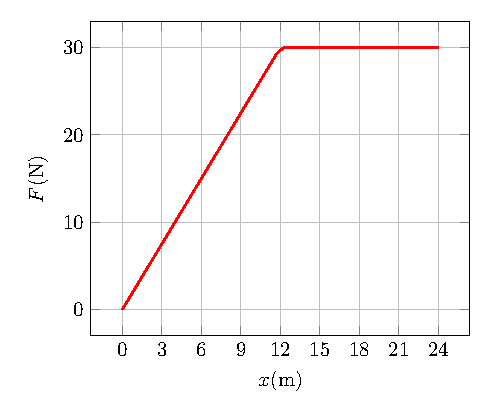
\includegraphics{hw-7-fig-1}
  \caption{Graph of the force $F$ with respect to distance.}
  \label{fig:hw-7-1}
\end{figure}
\end{problem}
\begin{proof}[Solution]
Remember that the work done by a force $F(x)$ over a distance
$a\leq x\leq b$ is given by the formula
\begin{equation}
  \label{eq:work}
W=\int_a^b F(x)\diff x.
\end{equation}
Since the graph in Figure (\ref{fig:hw-7-1}) is piecewise, all we need to
do is break up our interval $0\leq x\leq 24$ into the part where $y$ is a
diagonal line and where $y$ is a horizontal line, compute the work done on
each interval, $W_1$ and $W_2$, and add them up to get the total work
$W=W_1+W_2$.  First, note that over $0\leq x\leq 12$,
$F(x)=\frac{30}{12}x=\frac{5}{2}x$ so the work done from $0\leq x\leq 12$
is
\[
W_1=\int_0^{12}\frac{5}{2}x\diff x=
\left.\frac{5}{4}x^2\right|_0^{12}=
\frac{5}{4}(12)^2=\SI{180}{\joule}.
\]
Next, we see that $F(x)=30$ is constant for all $12\leq x\leq 24$
so we have
\[
W_2=\int_{12}^{24}F(x)\diff x=
\int_{12}^{24}30\diff x=
\left.30x\right|_{12}^{24}=
30\cdot 24-30\cdot 12=30\cdot 12=\SI{360}{\joule}.
\]
Hence, the total work done by $F(x)$ over $0\leq x\leq 24$ is
\[
  \boxed{W=W_1+W_2=\SI{180}{\joule}+\SI{360}{\joule}=\SI{540}{\joule}.}
\]
\end{proof}
\begin{problem}[WebAssign, HW8, 3]
A force of $6$ lb is required to hold a spring stretched $8$ in beyond its
natural length. How much work $W$ is done in stretching it from its natural
length to $14$ in beyond its natural length?
\end{problem}
\begin{proof}[Solution]
Recall \href{https://en.wikipedia.org/wiki/Hooke's_law}{Hooke's law} for
the force required to stretch a spring a distance $x$  beyond its natural
length
\begin{equation}
\label{eq:hookes-law}
F(x)=kx.
\end{equation}
Now, we are given a force of $6$ lb and a distance of $8$ in. Using this
information, we can figure out what the coefficient $k$ must be:
\[
k=F/x=6/8\mathrm{lb}/\mathrm{in}.
\]
Using the Equation (\ref{eq:work}) for work, we have that the work done on
a spring by stretching it from $x_1$ to $x_2$ is
\begin{equation}
\label{eq:work-on-spring}
W(x_1,x_2)=\int_{x_1}^{x_2}F(x)\diff x=\int_{x_1}^{x_2}kx\diff x=\left.\frac{1}{2}kx^2\right|_{x_1}^{x_2}=\frac{1}{2}k\left({x_1}^2-{x_2}^2\right)
\end{equation}
so, plugging in $14$, into our equation $W(x')$ above we get
\[
W(14)=\frac{1}{2}\cdot \frac{6}{8}\cdot
14^2=7\cdot\frac{6}{8}=\boxed{\frac{49}{8}\text{ ft-lb}.}
\]
\end{proof}
\begin{problem}[WebAssign, HW8, 4]
If the work required to stretch a spring $3$ ft beyond its natural length is
$9$ ft-lb, how much work is needed to stretch it $9$ in beyond its natural
length?
\end{problem}
\begin{proof}[Solution]
We employ the same idea as the one we used to calculate the work on the
last problem. First, we find the coefficient $k$, wit the help of Equation
(\ref{eq:work-on-spring}) this value will be
\[
k=\frac{2W}{x^2}=\frac{2\cdot 9}{9}=2\text{ lb}/\text{ft}.
\]
Now, convert our $9\text{ in}$ to ft we get $3/4\text{ ft}$. Lastly,
applying Equation (\ref{eq:work-on-spring}) on $3/4\text{ ft}$ we get
\[
W(3/4)=\frac{1}{2}\cdot 2\cdot (3/4)^2=\boxed{\frac{9}{16}\text{ in-lb}.}
\]
\end{proof}
\begin{problem}[WebAssign, HW8, 5]
An aquarium $\SI{6}{\meter}$ long, $\SI{1}{\meter}$ wide, and
$\SI{1}{\meter}$ deep is full of water. Find the work needed to pump half
of the water out of the aquarium. (Use $\SI{9.8}{\meter/\second^2}$ for $g$
and the fact that the density of water is
$\SI{1000}{\kilo\gram/\meter^3}$.)
\begin{itemize}
\item Show how to approximate the required work by a Riemann sum. (Let $x$
  be the height in meters below the top of the tank. Enter $x_i^*$ as $x_i$.)
\item Express the work as an integral.
\end{itemize}
\end{problem}
\begin{proof}[Solution]
Let's place the origin at the top of the tank. Then, the expression for the
work required to pump out half the water from our tank will be given
approximately by
\[
W(x)\approx\lim_{n\to\infty}\sum_{i=1}^n9.8\cdot1000\cdot 6\cdot x_i\Delta
x=\boxed{\sum_{i=1}^{n}58800 x_i^*\Delta x.}
\]
\\\\
Now we compute the integral from $0\leq x\leq 1/2$. We have
\[
W=58800\int_0^{1/2} x\diff x=5800\left(\left.\frac{1}{2}x^2\right|_0^{1/2} \right)=29400\left((1/2)^2-0\right)=\boxed{\SI{7350}{\joule}.}
\]
\end{proof}

\begin{problem}[WebAssign, HW8, 6]
A tank is full of water (see Figure \ref{fig:hw-7-2}). Find the work $W$
required to pump the water out of the spout. (Use
$\SI{9.8}{\meter/\second^2}$ for $g$. Use $\SI{1000}{\kilo\gram/\meter^3}$
as the weight density  of water. Assume that $a=\SI{4}{\meter}$,
$b=\SI{4}{\meter}$, $c=\SI{12}{\meter}$, and $d=\SI{2}{\meter}$.)
\begin{figure}[htbp]
  \centering
  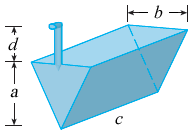
\includegraphics[scale=0.45]{hw-7-fig-2}
  \caption{A sketch of the tank.}
  \label{fig:hw-7-2}
\end{figure}
\end{problem}
\begin{proof}[Solution]
The work required to pump the water out of the spout of a tank with the
dimensions above is given by the
\[
W=\lim_{n\to\infty}\sum_{i=0}^n F(x_i)\Delta x
\]
where $\SI{0}{\meter}\leq x\leq\SI{8}{\meter}$. Now, the first thing we
need to do is to find the way the force changes as we move up the tank. Let
$x$ be the vertical distance from the bottom of the tank and $y$ be the
horizontal distance from. Then, the work needed to lift the slice slice of
volume $\Delta V$ that is a distance $(4+2)-x$ from the spout is
\begin{equation}
\label{eq:weight-density}
W(x)\approx g\rho(6-x)\Delta V,
\end{equation}
where $\rho$ is the density of the water and $g$ is gravity. Now, how does
our little slice of volume change as we move up the tank? If $y$ is the
side of the right-triangle made by going up a distance $x$ up the tank, then
\[
\frac{x}{y}=\frac{4}{4}=1
\]
since the triangles are similar. Hence, $y=2x$ so the volume change will be
\[
V(x)\approx 12\cdot\frac{1}{2}(2x)\Delta x=12x\Delta x(6-x),
\]
this is just the area of a triangle $x\Delta x$ (base times height) times
the depth $\SI{12}{\meter}$. Hence, the, plugging in the last equation into
our equation for the force (Equation (\ref{eq:weight-density})) will be
\[
W(x)\approx g\rho(6-x)\left(12 x\Delta x\right)=117600(6-x)x\Delta x
\]
Last but not least, we compute the limit as
$n\to\infty$,
\begin{align*}
W&=\lim_{n\to\infty}\sum_{i=0}^n W(x_i)\Delta x\\
\shortintertext{this is just the integral}
 &=117600\int_0^4(6-x)x\diff x\\
 &=117600\int_0^46x-x^2\diff x\\
 &=117600\left(\left.3x^2-\frac{1}{3}x^3\right|_0^4\right)\\
 &=117600\left(3\cdot 4^2-\frac{4^3}{3}-(0-0)\right)\\
 &=117600\left(\frac{3\cdot 3\cdot 4^2-4^3}{3}\right)\\
 &=117600\left(4^2\cdot\frac{9-4}{3}\right)\\
 &=117600\left(4^2\cdot\frac{5}{3}\right)\\
 &=\boxed{\SI{3136000}{\joule}.}
\end{align*}
\end{proof}
% p453:11,14
\begin{problem}[WebAssign, HW8, 7]
Consider the given function and the given interval
\[
f(x)=10\sin x-5\sin 2x,\quad[0,\pi]
\]
\begin{enumerate}[label=(\alph*)]
\item Find the average value $f_{\text{ave}}$ of $f$ on the given
  interval.
\item Find $c$ such that $f_{\text{ave}}=f(c)$.
\item Sketch the graph of $f$ and a rectangle whose area is the same as the
  area under the graph of $f$.
\end{enumerate}
\end{problem}
\begin{proof}[Solution]
(a) Recall the definition of the average of a function over an interval
$[a,b]$, it is
\begin{equation}
  \label{eq:average}
f_{\text{ave}}=\frac{1}{b-a}\int_a^b f\diff x.
\end{equation}
Now, all we need to do is calculate the integral of our $f$ and divide that
value by $\pi-0$, i.e.,
\begingroup
\allowdisplaybreaks
\begin{align*}
f_{\text{ave}}&=\frac{1}{\pi}\int_0^\pi f(x)\diff x\\
&=\frac{1}{\pi}\int_0^\pi 10\sin x-5\sin 2x\diff x\\
&=\frac{1}{\pi}\left(\left.-10\cos x+\frac{5}{2}\cos
  2x\right|_0^\pi\right)\\
&=\frac{1}{\pi}\left(-10\cos\pi+\frac{5}{2}\cos 2\pi-\left(-10\cos
  0+\frac{5}{2}\cos 0\right)\right)\\
&=\frac{1}{\pi}\left(10+\frac{5}{2}+10-\frac{5}{2}\right)\\
&=\frac{1}{\pi}\cdot 20\\
&=\boxed{\frac{20}{\pi}.}
\end{align*}
\endgroup
\\\\
(b) For this part all we need to do is set the equation $f(x)=10\sin
x-5\sin 2x$ equal to $20/\pi$ and solve for $x$:
\[
10\sin x-5\sin 2x=5(2\sin x-\sin 2x)=\frac{20}{\pi}
\]
so
\[
  2\sin x-\sin 2x=\frac{4}{\pi}.
\]
I can't think of any way to solve this than plugging it into your
calculator and having your calculator approximate the solution (your
calculator probably uses
\href{https://en.wikipedia.org/wiki/Newton's_method}{Newton's method},
which you will learn about later in your career). The values are about
\ul{$c\approx 1.238$ and $2.808$.}
\\\\
(c) Sketching the graph is easy and the box having the same area as will
have height equal to $20/\pi$ and length $\pi$. Multiply these together and
we get the area under the curve, which we computed to be $20$.
\end{proof}
\begin{problem}[WebAssign, HW8, 8]
Find the numbers b such that the average value of
$f(x)=7+10x-9x^2$ on the interval $[0,b]$ is equal to $8$.
\end{problem}
\begin{proof}[Solution]
This exercise is easy-peasy :-). All you need to do is compute the average
\[
f_\text{ave}=\frac{1}{b-0}\int_0^b7+10x-9x^2\diff x=7+5b-3b^2.
\]
Now, set the above equal to $8$ and we have
\[
7+5b-3b^2=8
\]
and solve for $b$. We get \ul{$b=(5-\sqrt{13})/6$ or $(5+\sqrt{13})/6$.}
\end{proof}

%%% Local Variables:
%%% mode: latex
%%% TeX-master: "../MA166-HW-Current"
%%% End:

\chapter{Homework 9 Solutions}
\begin{problem}[WebAssign HW 9, 1]
Evaluate the integral using integration by parts with the indicated choices
of $u$ and $\diff v$. (Use $C$ for the constant of integration.)
\[
\int 7x^2\ln x\diff x;\qquad
u=\ln x,\quad
\diff v=7x^2\diff x.
\]
\end{problem}
\begin{proof}[Solution]
Remember the formula for integration by parts? No? Well, here it is:
\begin{equation}
  \label{eq:integration-by-parts}
\int u\diff v=uv-\int v\diff u.
\end{equation}
Now, let us integrate the above expression making the substitutions which
were given to us:
\begin{align*}
\int u\diff v&=\int\ln 7x^2\diff x\\
             &=\tfrac{7}{3}x^3\ln x-\int\frac{1}{x}\cdot \tfrac{7}{3}x^3\diff
               x\\
             &=\tfrac{7}{3}x^3\ln x-\int \tfrac{7}{3}x^2 \diff x\\
             &=\boxed{\tfrac{7}{3}x^3\ln x-\tfrac{7}{9}x^3+C}
\end{align*}
\end{proof}

\begin{problem}[WebAssign HW 9, 2]
Evaluate the integral. (Use $C$ for the constant of integration.)
\[
\int 5x\cos 6x\diff x.
\]
\end{problem}
\begin{proof}[Solution]
Since the derivative of $5x$ is just $5$, let's use the substitution $u=5x$
and $\diff v=\cos 6x\diff x$. Then, substituting this into Equation
(\ref{eq:integration-by-parts}) we have:
\begin{align*}
  \int u\diff v&=\int 5x\cos 6x\diff x\\
               &=\tfrac{5}{6}x\sin 6x-\int \tfrac{5}{6}\sin 6x\diff x\\
               &=\boxed{\tfrac{25}{6}x\sin 6x+\tfrac{5}{36}\cos 6x+C.}
\end{align*}
\end{proof}

\begin{problem}[WebAssign HW 9, 3]
Evaluate the integral. (Use $C$ for the constant of integration.)
\[
\int \left( x^2+3x \right)\cos x\diff x.
\]
\end{problem}
\begin{proof}[Solution]
Again, since the third derivative of $x^2+3x$ disappears, let's make make
the substitution $u=x^2+3x$ and $\diff v=\cos x\diff x$. Then, we have
\begin{align}
\label{eq:hw-9-3}
\int u\diff v
&=\int \left(x^2+3\right)\cos x\diff x\nonumber\\
&=\left(x^2+3x\right)\sin x-\int (2x+3)\sin x\diff x.
\end{align}
Now what? That second integral looks pretty hard to integrate? We use
integration by parts on that. Since the derivative of $2x$ is $2$ let's
make the substitution $u=2x$ and $\diff v=\sin x\diff x$ and we have
\[
\int (2x+3)\sin x\diff x=
-(2x+3)\cos x-\int 2(-\cos x)\diff x
=-(2x+3)\cos x+2\sin x.
\]
Substituting this back into Equation (\ref{eq:hw-9-3}), we have
\begin{align*}
\int u\diff v
&=\left(x^2+3x\right)\sin x-\int 2x\sin x\diff x\\
&=\left(x^2+3x\right)\sin x-\left(-(2x+3)\cos x+2\sin x\right)\\
&=\left(x^2+3x\right)\sin x+(2x+3)\cos x-2\sin x+C\\
&=\boxed{\left(x^2+3x-2\right)\sin x+(2x+3)\cos x+C.}
\end{align*}
\end{proof}

\begin{problem}[WebAssign HW 9, 4]
Evaluate the integral. (Use $C$ for the constant of integration.)
\[
\int\sin^{-1}x\diff x
\]
\end{problem}
\begin{proof}[Solution]
If it were not for integration by parts, I wouldn't know how to even begin
to integrate this one. Since we know the derivative of $\sin^{-1}x$, let's
make the substitution $u=\sin^{-1}x$ and $\diff v=\diff x$. Then we have
\begin{align*}
\int u\diff v&=\int \sin^{-1}x\diff x\\
             &=x\sin^{-1}x-\int\frac{x}{\sqrt{1-x^2}}\diff x.
\end{align*}
Now, how in the world do we evaluate $\int\frac{x}{\sqrt{1-x^2}}\diff x$?
Integration by parts? That sounds hard. Why not make a substitution? What
substitution? Well, we have a power of $x$ in the denominator of the
integral
\[
\int\frac{x}{\sqrt{1-x^2}}\diff x,
\]
and we have a square root of a $x^2$ in the denominator, why not $w=1-x^2$?
If we do that, we have $\diff w=-2x\diff x$,i.e., $\diff x=\diff w/(-2x)$
and we have
\begingroup
\allowdisplaybreaks
\begin{align*}
\int\frac{x}{\sqrt{w}}\frac{\diff w}{-2x}
&=\int\frac{1}{-2\sqrt{w}}\diff w\\
&=-\frac{1}{2}\int w^{-1/2}\diff w\\
&=-\frac{1}{2}\left(\frac{w^{1/2}}{1/2}\right)\\
&=w^{1/2}\\
&=\sqrt{1-x^2.}
\end{align*}
\endgroup
Now, back to our original problem. Substituting what we just computed, we
have
\[
\int \sin^{-1}x\diff x=\boxed{x\sin^{-1}x-\sqrt{1-x^2}+C.}
\]
\end{proof}

% p468:1,3,7,10,17,27,29,32,37,62
\begin{problem}[WebAssign HW 9, 5]
Evaluate the integral.
\[
\int_1^3 17r^3\ln r\diff r.
\]
\end{problem}
\begin{proof}[Solution]
Hopefully, you have caught on the pattern here. We make a choice of $u$ and
$\diff v$ depending on which one we think is easier to differentiate or
integrate. In this case, the integral of $\ln r$ is hard, but the integral
of $17r^3$ is easy so let's make the substitution $u=\ln r$ and $\diff
v=17r^3\diff x$ and we get
\begin{align*}
  \int_1^3 u\diff v&=\int_1^3 17r^3\ln r\diff r\\
                   &=\left.\tfrac{17}{4}r^4\ln r\right|_1^3
                     -\int_1^3\frac{17r^4}{4r}\diff r\\
                   &=\left.\tfrac{17}{4}r^4\ln
                     r-\tfrac{17}{16}r^4\right|_1^3\\
                   &=\left.\frac{4\cdot 17r^4\ln
                     r-17r^4}{16}\right|_1^3\\
                   &=\left.\frac{17r^4(4\ln r-1)}{16}\right|_1^3\\
                   &=\frac{17\cdot 3^4(4\ln 3-1)}{16}-\frac{17\cdot (4\ln
                     1-1)}{16}\\
                   &=\frac{1377(4\ln 3-1)}{16}+\frac{17}{16}\\
                   &=\frac{1377\cdot 4\ln 3-1377+17}{16}\\
                   &=\tfrac{1377}{4}\ln 3-\tfrac{1360}{16}\\
                   &=\boxed{\tfrac{1377}{4}\ln 3-85.}
\end{align*}
\end{proof}

\begin{problem}[WebAssign HW 9, 6]
Evaluate the integral.
\[
\int_0^1 \frac{y}{e^{3y}}\diff y.
\]
\end{problem}
\begin{proof}[Solution]
By parts, let $u=y$ and $\diff v=e^{-3y}\diff y$. Then, we have
\begin{align*}
\int_0^1\frac{y}{e^{3y}}\diff y
&=\left.-\frac{ye^{-3y}}{3}\right|_0^1-\int-\frac{e^{-3y}}{3}\diff y\\
&=\left.-\frac{ye^{-3y}}{3}\right|_0^1
+\int\frac{e^{-3y}}{3}\diff y\\
&=\left.-\frac{ye^{-3y}}{3}-\frac{e^{-3y}}{9}\right|_0^1\\
&=\left.-\frac{3ye^{-3y}+e^{-3y}}{9}\right|_0^1\\
&=-\frac{3e^{-3}+e^{-3}}{9}+\frac{1}{9}\\
&=\boxed{\frac{1-4e^{-3}}{9}.}
\end{align*}
\end{proof}

\begin{problem}[WebAssign HW 9, 7]
Evaluate the integral.
\[
\int_1^5\frac{\ln^2 x}{x^3}\diff x.
\]
\end{problem}
\begin{proof}[Solution]
First, make the substitution $u=\ln^2 x$ and $\diff v=\diff x/x^3$. Then,
we have
\begin{align*}
\int u\diff v&=\int_1^5\frac{\ln^2 x}{x^3}\diff x\\
             &=\left.-\frac{\ln^2 x}{2x^2}\right|_1^5
               -\int_1^5-\frac{2\ln x}{2x^3}\diff x\\
             &=\left.-\frac{\ln^2 x}{2x^2}\right|_1^5
               +\int_1^5\frac{\ln x}{x^3}\diff x.
\end{align*}
Then we integrate $\int_1^5-\ln x/x^3\diff x$ by parts and we get
\begin{align*}
\int_1^5\frac{\ln x}{x^3}\diff x
&=\left.-\frac{\ln x}{2x^2}\right|_1^5
+\int_1^5\frac{1}{x}\frac{1}{2x^2}\diff x\\
&=\left.-\frac{\ln x}{2x^2}\right|_1^5
+\int_1^5\frac{1}{2x^3}\diff x\\
&=\left.-\frac{\ln x}{2x^2}-\frac{1}{4x^2}\right|_1^5\\
&=\left.-\frac{2\ln x+1}{4x^2}\right|_1^5.
\end{align*}
So our integral is
\begin{align*}
\left.-\frac{\ln^2 x}{2x^2}-\frac{2\ln x+1}{4x^2}\right|_1^5
&=\left.-\frac{2\ln^2 x+2\ln x+1}{4x^2}\right|_1^5\\
&=-\frac{2\ln^2 5+2\ln 5+1}{4\cdot 5^2}+\frac{1}{4}\\
&=-\frac{2\ln^2 5+2\ln 5-24}{4\cdot 5^2}\\
&=\boxed{\frac{6}{25}-\tfrac{1}{50}\ln^2 5-\tfrac{1}{50}\ln 5.}
\end{align*}
\end{proof}

\begin{problem}[WebAssign HW 9, 8]
First make a substitution and then use integration by parts to evaluate the
integral. (Use $C$ for the constant of integration.)
\[
\int 7\cos\sqrt{x}\diff x.
\]
\end{problem}
\begin{proof}
What's the most obvious substitution? Perhaps $w=\sqrt{x}$. Then, we get
\[\diff w=-\frac{\diff x}{2\sqrt{x}}=\frac{\diff x}{2w}.\]
So our integral turns into
\[
\int 14 w\cos w\diff w
\]
Then, by integration by parts, setting $u=14w$, we get
\begin{align*}
  \int u\diff v&=\int 14w\cos w\diff w\\
               &=14w\sin w-\int 14\sin w\diff w\\
               &=14w\sin w-\int 14\sin w\diff w\\
               &=14w\sin w+14\cos w+C.
\end{align*}
Substituting back, we get our answer
\[
\boxed{14\sqrt{x}\sin\sqrt{x}+14\cos\sqrt{x}+C.}
\]
\end{proof}

\begin{problem}[WebAssign HW 9, 9]
Use the method of cylindrical shells to find the volume $V$ generated by
rotating the region bounded by the given curves about the specified axis.
\[
y=4e^x,\quad y=4e^{-x},\quad x=1;\qquad\text{about the $y$-axis.}
\]
\end{problem}
\begin{proof}[Solution]
I give up on trying to plot these, (it's too much work for one person). By
the method of cylindrical shells, we want to find an expression for the
cross-sectional area (which has the form of a cylinder) in terms of our
variable perpendicular to the axis we are rotating about. In this case, we
are rotating about the $y$-axis, so we must solve for the cross-sectional
area in terms of $x$ like so:
\[
A(x)=2\pi x(4e^x-4e^{-x})=8\pi x(e^{x}-e^{-x}).
\]
Then, we integrate the area between where the curves $4e^x$, $4e^{-x}$ and
$x=1$ intersect (if you plot the curves, this will be the area of the
difference of $e^x$ and $e^{-x}$ from $0\leq x\leq 1$). Thus, the
volume is
\begin{align*}
V&=\int_0^1 8\pi x(e^x-e^{-x})\diff x\\
 &=8\pi\left(\left.x(e^x+e^{-x})\right|_0^1
   -\int_0^1 e^x+e^{-x}\diff x\right)\\
 &=8\pi\left(\left.x(e^x+e^{-x})\right|_0^1
   -\int_0^1 e^x+e^{-x}\diff x\right)\\
 &=8\pi\left(\left. x(e^x+e^{-x})-e^x+e^{-x}\right|_0^1\right)\\
 &=8\pi\left(e+e^{-1}-e+e^{-1}-(0-1+1)\right)\\
 &=\boxed{\frac{16\pi}{e}.}
\end{align*}
\end{proof}

%%% Local Variables:
%%% mode: latex
%%% TeX-master: "../MA166-HW-Current"
%%% End:

\chapter{Homework 10 Solutions}
\begin{problem}[WebAssign HW 10, 1]
Evaluate the integral. (Use $C$ for the constant of integration.)
\[
\int 2\sin^2 x\cos^3 x\diff x
\]
\end{problem}
\begin{proof}[Solution]
First, note that $\cos^2 x=1-\sin^2 x$ so the integral above can be written
as
\begin{align*}
\int 2\sin^2 x\cos^3 x\diff x
&=\int 2\sin^2 x\cos^2 x\cos x\diff x\\
&=\int 2\sin^2x(1-\sin^2 x)\cos x\diff x.
\end{align*}
Now, make the substitution $u=\sin x$. Then $\diff u=\cos x\diff x$ so our
integral is now
\begin{align*}
\int 2u^2(1-u^2)\cos x\frac{\diff u}{\cos x}
&=\int 2u^2(1-u^2)\diff u\\
&=\int 2u^2-2u^4\diff u\\
&=\tfrac{2}{3}u^3-\tfrac{2}{5}u^5+C\\
&=\boxed{\tfrac{2}{3}\sin^3 x-\tfrac{2}{5}\sin^5 x+C.}
\end{align*}
\end{proof}

\begin{problem}[WebAssign HW 10, 2]
Evaluate the integral
\[
\int_0^{\pi/2}5\cos^2\theta\diff\theta.
\]
\end{problem}
\begin{proof}[Solution]
For this problem, we can use the double-angle identity, i.e.,
\begin{equation}
  \label{eq:cosine-double-angle}
\cos 2\theta=2\cos^2\theta-1=1-2\sin^2 x
\end{equation}
Substituting Equation (\ref{eq:cosine-double-angle}) into our integral, we
have
\begin{align*}
\int_0^{\pi/2}5\cos^2\theta\diff\theta&=
\int_0^{\pi/2}\tfrac{5}{2}(1+\cos 2\theta)\diff\theta\\
&=\tfrac{5}{2}\int_0^{\pi/2}(1+\cos 2\theta)\diff\theta\\
&=\tfrac{5}{2}\left(\left.\theta+\tfrac{1}{2}\sin
  2\theta\right|_0^{\pi/2}\right)\\
&=\tfrac{5}{2}\left(\frac{\pi}{2}+0-(0+0)\right)\\
&=\boxed{\frac{5\pi}{4}.}
\end{align*}
\end{proof}

\begin{problem}[WebAssign HW 10, 3]
Evaluate the integral.
\[
\int_0^{\pi/2}5\sin^2 x\cos^2 x\diff x.
\]
\end{problem}
\begin{proof}[Solution]
Again, we just use a trigonometric identity, specifically
\begin{equation}
  \label{eq:sine-double-angle}
\sin 2 x =2\sin  x \cos x .
\end{equation}
Using Equation (\ref{eq:sine-double-angle}) our integral turns into
\begin{align*}
\int_0^{\pi/2}5\sin^2x\cos^2x\diff x
&=5\int_0^{\pi/2}\tfrac{1}{4}(4\sin^2 x\cos^2x)\diff x\\
&=\frac{5}{4}\int_0^{\pi/2}(2\sin x\cos x)^2\diff x\\
&=\frac{5}{4}\int_0^{\pi/2}(\sin 2x)^2\diff x\\
&=\frac{5}{4}\int_0^{\pi/2}\sin^2 2x\diff x\\
&=\frac{5}{4}\int_0^{\pi/2}\sin^2 2x\diff x\\
\shortintertext{now we use this identity $2\sin^2 x =1-\cos 2 x $
  to get}
&=\frac{5}{4}\int_0^{\pi/2}\frac{1}{2}(1-\cos 4 x )\diff x \\
&=\frac{5}{8}\int_0^{\pi/2}1-\cos 4 x \diff x \\
&=\frac{5}{8}\left(\left. x -\tfrac{1}{4}\sin
  4 x \right|_0^{\pi/2}\right)\\
&=\boxed{\tfrac{5\pi}{16}.}
\end{align*}
\end{proof}

\begin{problem}[WebAssign HW 10, 4]
Evaluate the integral. (Remember to use $\ln(|u|)$ where appropriate. Use
$C$ for constant of integration.)
\[
\int 9\cos^2 x\tan^3 x\diff x.
\]
\end{problem}
\begin{proof}[Solution]
Let's make the substitution $u=\cos x$ so $\diff u=-\sin x\diff x$ and we
have
\begingroup
\allowdisplaybreaks
\begin{align*}
\int 9\cos^2 x\tan^3 x\diff x
&=9\int \cos^2 x\tan^3 x\diff x\\
&=9\int\frac{\cos^2 x\sin^3 x}{\cos^3 x}\diff x\\
&=9\int\frac{\sin^3 x}{\cos x}\diff x\\
&=9\int\frac{\sin x(1-\cos^2 x)}{\cos x}\diff x\\
\shortintertext{now, for the substitution,}
&=9\int\frac{\sin x(1-u^2)}{u}\frac{\diff u}{-\sin x}\\
&=9\int\frac{u^2-1}{u}\diff u\\
&=9\int u-\frac{1}{u}\diff u\\
&=\tfrac{9}{2}u^2-9\ln|u|+C\\
\shortintertext{and back, we have}
&=\boxed{\tfrac{9}{2}\cos^2 x-9\ln|\cos x|+C.}
\end{align*}
\endgroup
\end{proof}

\begin{problem}[WebAssign HW 10, 5]
Evaluate the integral. (Use $C$ for the constant of integration.)
\[
\int 5\tan^2 x\diff x.
\]
\end{problem}
\begin{proof}[Solution]
The easiest one so far. Recall the identity
\begin{equation}
  \label{eq:tangent-identity}
\sec^2 x -\tan^2 x =1.
\end{equation}
Then, we gave
\[
\int 5\tan^2x\diff x=5\int(\sec^2 x -1)\diff x =
\boxed{5\tan x -5 x +C.}
\]
\end{proof}

% p476:1,7,11,17,23,24,35,61
\begin{problem}[WebAssign HW 10, 6]
\[
\int 8\left(\tan^2x+\tan^4x\right)\diff x.
\]
\end{problem}
\begin{proof}[Solution]
We'll make the substitution $u=\tan x$, so $\diff u=\sec^2x\diff
x$. Proceeding, we have
\begin{align*}
\int 8\left(\tan^2 x+\tan^4x\right)\diff x
&=8\int\tan^2 x(1+\tan^2 x)\diff x\\
\shortintertext{by Equation (\ref{eq:tangent-identity}), we have}
&=8\int\tan^2 x\sec^2 x\diff x\\
&=8\int u^2\diff u\\
&=\tfrac{8}{3}u^3+C\\
&=\boxed{\tfrac{8}{3}\tan^3 x+C.}
\end{align*}
\end{proof}

\begin{problem}[WebAssign HW 10, 7]
Evaluate the integral
\[
\int_{\pi/6}^{\pi/2}\cot^2 x\diff x
\]
\end{problem}
\begin{proof}[Solution]
Remember that, like Equation (\ref{eq:tangent-identity}), there is a
cotangent-identity
\begin{equation}
  \label{eq:cotangent-identity}
1+\cot^2 x=\csc^2 x.
\end{equation}
With the help of this equation, we have
\begin{align*}
\int_{\pi/6}^{\pi/2}\cot^2 x\diff x&=
\int_{\pi/6}^{\pi/2}(\csc^2-1)\diff x\\
&=\left.-\cot x-x\right|_{\pi/6}^{\pi/2}\\
&=0-\frac{\pi}{2}-\left(\sqrt{3}-\frac{\pi}{6}\right)\\
&=\boxed{\sqrt{3}-\frac{\pi}{3}.}
\end{align*}
\end{proof}

\begin{problem}[WebAssign HW 10, 8]
Find the volume $V$ obtained by rotating the region bounded by the given
curves about the specified axis.
\[
y=9\sin x,\quad
y=0,\quad
\frac{\pi}{2}\leq x\leq\pi;\qquad
\text{about the $x$-axis.}
\]
\end{problem}
\begin{proof}[Solution]
Since we are rotating about the $x$-axis, we need to find the
cross-sectional area in terms of $y$ in terms of $x$, hence we have
\[
A(x)=\pi y^2=81\pi\sin^2 x.
\]
Now, integrating from $\pi/2$ to $\pi$, we get
\begin{align*}
\int_{\pi/2}^\pi A(x)\diff x
&=81\pi\int_{\pi/2}^\pi \sin^2 x\\
\shortintertext{using the double-angle identity for cosine, Equation
  (\ref{eq:cosine-double-angle}), we get}
&=81\pi\int_{\pi/2}^\pi \tfrac{1}{2}(1-\cos 2x)\diff x\\
&=\tfrac{81\pi}{2}\left(\left.x-\tfrac{1}{2}\sin 2x\right|_{\pi/2}^\pi\right)\\
&=\tfrac{81\pi}{2}\left(\pi-0-(\tfrac{1}{2}\pi)\right)\\
&=\boxed{\frac{81\pi^2}{4}.}
\end{align*}
\end{proof}

%%% Local Variables:
%%% mode: latex
%%% TeX-master: "../MA166-HW-Current"
%%% End:

\end{document}

%%% Local Variables:
%%% mode: latex
%%% TeX-master: t
%%% End:
